\documentclass{scrartcl}
\usepackage[a4paper,left=1in,right=1in,top=1.2in,bottom=1in]{geometry}
\usepackage{siunitx}
\usepackage{graphicx}
\usepackage{textcomp}
\usepackage{amsmath}
\usepackage{mathtools}
\newcommand*\diff{\mathop{}\!\mathrm{d}}
\newcommand*\Diff[1]{\mathop{}\!\mathrm{d^#1}}
\setkomafont{disposition}{\normalfont\bfseries}

%title
\title{Exercise 04:\\Hodgkin-Huxley model}
\subtitle{Theoretical Neuroscience I}
\author{Maria del Cerro \and Johannes G\"atjen \and Lorena Morton}

%use these for structure/overview
\newcommand\Question{%
  \textbf{Question:}%
}
\newcommand\Answer{%
  \textbf{Answer:}%
}

\begin{document}
\maketitle
\section{Analytic derivation}

Start from
\begin{equation*}
c_m\frac{\diff V}{\diff t} = -i_\mathrm{L}-i_\mathrm{Na} -i_\mathrm{K} + i_e.
\end{equation*}
The different parts of the membrane current
\begin{equation*}
i_\mathrm{L} = g_\mathrm{L}(V-E_\mathrm{L}) \qquad i_\mathrm{Na} = g_\mathrm{Na}m^3h(V-E_\mathrm{Na}) \qquad i_\mathrm{K} = g_\mathrm{K}n^4(V-E_\mathrm{K})
\end{equation*}
can be substituted with the respective conductance times driving force:
\begin{align*}
c_m\frac{\diff V}{\diff t} &= -g_\mathrm{L}(V-E_\mathrm{L}) - g_\mathrm{Na}m^3h(V-E_\mathrm{Na}) - g_\mathrm{K}n^4(V-E_\mathrm{K}) + i_e\\
\shortintertext{Factorize and sort according to $V$\dots}
&= -g_\mathrm{L}V  - g_\mathrm{Na}m^3h V - g_\mathrm{K}n^4 V + g_\mathrm{L}E_\mathrm{L} + g_\mathrm{Na}m^3hE_\mathrm{Na}+ g_\mathrm{K}n^4E_\mathrm{K} + i_e\\
\shortintertext{\dots so that we can factorize $-V$\dots}
&= -V \left(g_\mathrm{L} + g_\mathrm{Na}m^3h + g_\mathrm{K}n^4\right) + g_\mathrm{L}E_\mathrm{L} + g_\mathrm{Na}m^3hE_\mathrm{Na}+ g_\mathrm{K}n^4E_\mathrm{K} + i_e\\
\shortintertext{\dots and factorize $\left(g_\mathrm{L} + g_\mathrm{Na}m^3h + g_\mathrm{K}n^4\right)$\dots}
&= \left(g_\mathrm{L} + g_\mathrm{Na}m^3h + g_\mathrm{K}n^4\right)\left(\frac{g_\mathrm{L}E_\mathrm{L} + g_\mathrm{Na}m^3hE_\mathrm{Na}+ g_\mathrm{K}n^4E_\mathrm{K} + i_e}{g_\mathrm{L} + g_\mathrm{Na}m^3h + g_\mathrm{K}n^4} - V\right)\\
\shortintertext{\dots and finally divide everything by $c_m$.}
\frac{\diff V}{\diff t} &= \frac{g_\mathrm{L} + g_\mathrm{Na}m^3h + g_\mathrm{K}n^4}{c_m}\left(\frac{g_\mathrm{L}E_\mathrm{L} + g_\mathrm{Na}m^3hE_\mathrm{Na}+ g_\mathrm{K}n^4E_\mathrm{K} + i_e}{g_\mathrm{L} + g_\mathrm{Na}m^3h + g_\mathrm{K}n^4} - V\right)\\
\end{align*}
With
\begin{equation*}
\tau_\mathrm{eff} = \frac{c_m}{g_\mathrm{L} + g_\mathrm{Na}m^3h + g_\mathrm{K}n^4} \quad \text{and} \quad V_\infty^\mathrm{eff} = \frac{g_\mathrm{L}E_\mathrm{L} + g_\mathrm{Na}m^3hE_\mathrm{Na}+ g_\mathrm{K}n^4E_\mathrm{K} + i_e}{g_\mathrm{L} + g_\mathrm{Na}m^3h + g_\mathrm{K}n^4}
\end{equation*}
this is equal to
\begin{equation*}
\frac{\diff V}{\diff t} = \frac{1}{\tau_\mathrm{eff}}\left(V_\infty^\mathrm{eff} - V\right)
\end{equation*}

\section{Simulation of neurons}
We start by simulating a neuron without an input current in order to observe the resting state (steady state) of the neuron. The time courses of the state variables are shown in Figure \ref{zero}. The membrane voltage, as well as the $n$ and $m$ gating variables relax close to their steady state values within a few \si{ms}. The inactivation variable $h$ on the other hand takes considerably longer to reach its equilibrium value (approx. 18\si{ms} to get to $90\%$ of the final value).

Now we use the steady state of the neuron as the initial state for a neuron with a large constant input current of $100 \si{\nano\ampere\per\square\milli\meter}$ (Figure \ref{large}). Within $40 \si{ms}$ we can observe three action potentials. The first action potential has a slightly larger amplitude than the other two, who appear equal in size.

During an action potential the membrane potential rises within a few \si{ms} to $\sim$30--40 \si{mV} (depolarization), then falls just as quickly to around $-75 \si{mV}$, which is 10 \si{mV} below the resting potential of $-65\si{mV}$ (repolarization and hyperpolarization). After this the membrane potential rises slowly, almost linearly, until it reaches a threshold value (approx. $-50 \si{mV}$) at which point another action potential is initiated. At the beginning of an action potential the sodium activation gates $m$ open very quickly, then stay almost completely open for a few \si{ms} before closing very quickly again. The sodium inactivation gates $h$ close more slowly than the $m$ gates open and after the action potential is over only gradually reopen. The potassium gates $n$ operate on a similar time scale is the $h$ gates but open first, then gradually close again.

Next we use a different initial state for the neuron and an intermediate constant input current of $62 \si{\nano\ampere\per\square\milli\meter}$ (Figure \ref{med}). Two action potentials are generated within 40\si{ms}. They have a slightly lower amplitude than the action potentials generated with the large input current, but otherwise the time courses do not differ much after the membrane has crossed a certain threshold.

Finally, a slightly lower constant input current of $61 \si{\nano\ampere\per\square\milli\meter}$ is used (Figure \ref{med_minus}). Here only a single action potential is generated, as the membrane potential decreases again, before it reaches the threshold value. Apparently this is due to the fact, that as the membrane voltage rises slowly the sodium inactivation gates close and the  enough to prohibit the strong sodium influx necessary for an action potential.

We can see, that with the interaction of just four dynamic variables, the Hodgkin-Huxley model exhibits many of the properties of a real neuron:
\begin{itemize}
\item The characteristic time course of an action potential with depolarization, repolarization and hyperpolarization.
\item Voltage-dependent firing rates.
\item A refractory period, in which no additional action potentials can be elicited.
\item An implicit threshold potential, above which the action potential is triggered.
\item Repeated action potentials are more difficult to elicit and have a smaller amplitude.
\end{itemize}

\begin{figure}
\centering
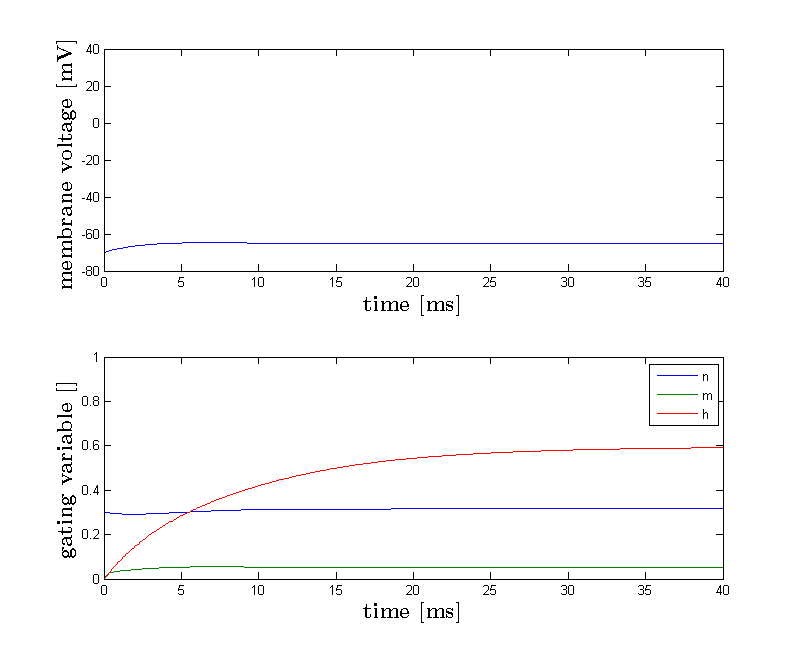
\includegraphics[trim = {1.4cm 0.3 1.8cm 1cm}, height=0.35\textheight, clip]{../pics/zero}
\caption{No input current. Initial condition: $V_0 = -70\si{mV}, n_0 = 0.3, m_0 = h_0 = 0$. Top:~Membrane voltage over time. Bottom: Gating variables $n, m$ and $h$ over time.}
\label{zero}
\end{figure}

\begin{figure}
\centering
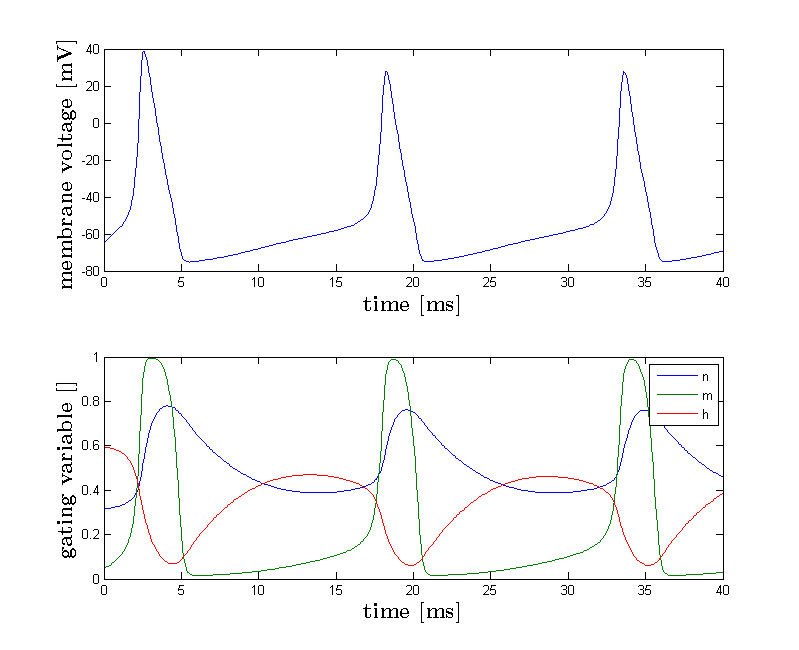
\includegraphics[trim = {1.4cm 0.3 1.8cm 1cm}, height=0.35\textheight, clip]{../pics/large}
\caption{Constant input current of $100 \si{\nano\ampere\per\square\milli\meter}$. The initial condition is equal to the steady state condition of the neuron with zero input current (see Figure \ref{zero}). Top: Membrane voltage over time. Bottom: Gating variables $n, m$ and $h$ over time.}
\label{large}
\end{figure}

\begin{figure}
\centering
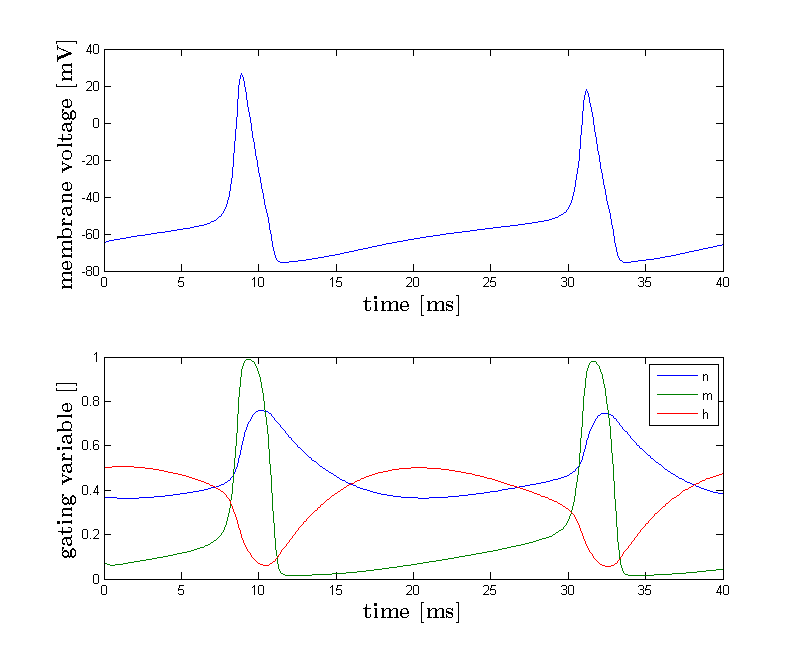
\includegraphics[trim = {1.4cm 0.3 1.8cm 1cm}, height=0.35\textheight, clip]{../pics/med}
\caption{Constant input current of $62 \si{\nano\ampere\per\square\milli\meter}$. Initial condition: $V_0=-65\si{mV}$, $n_0=0.37$, $m_0=0.08$, $h_0 = 0.5$. Top:~Membrane voltage over time. Bottom: Gating variables $n, m$ and $h$ over time.}
\label{med}
\end{figure}

\begin{figure}
\centering
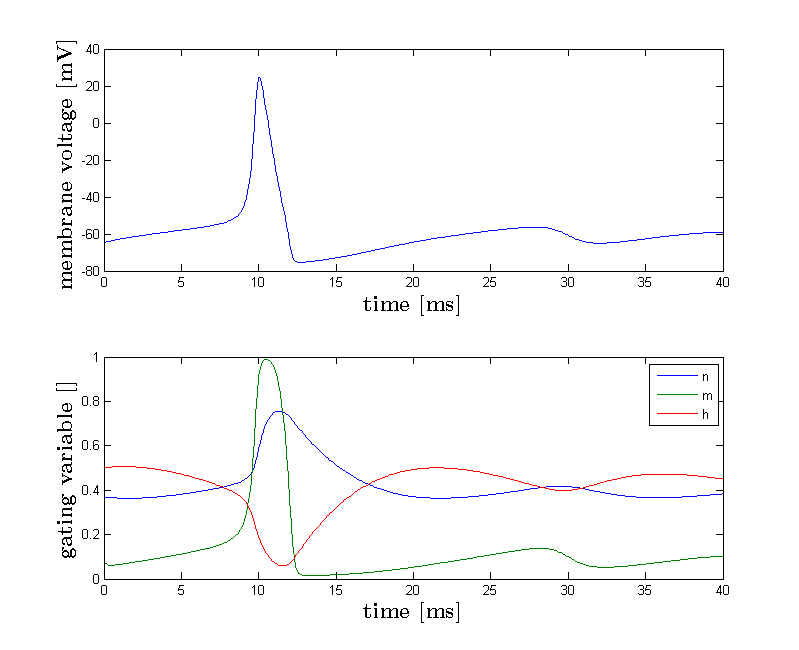
\includegraphics[trim = {1.4cm 0.3 1.8cm 1cm}, height=0.35\textheight, clip]{../pics/med_minus}
\caption{Constant input current of $61 \si{\nano\ampere\per\square\milli\meter}$. Initial condition: $V_0 = -65\si{mV}$, $n_0 = 0.37$, $m_0 = 0.08$, $h_0 = 0.5$. Top: Membrane voltage over time. Bottom: Gating variables $n, m$ and $h$ over time.}
\label{med_minus}
\end{figure}

\end{document}